\section{Описание модели}
	Структурная схема модели представленна на рисунке \ref{pic:scheme}.
	
	\begin{figure}[h]
		\begin{center}
			{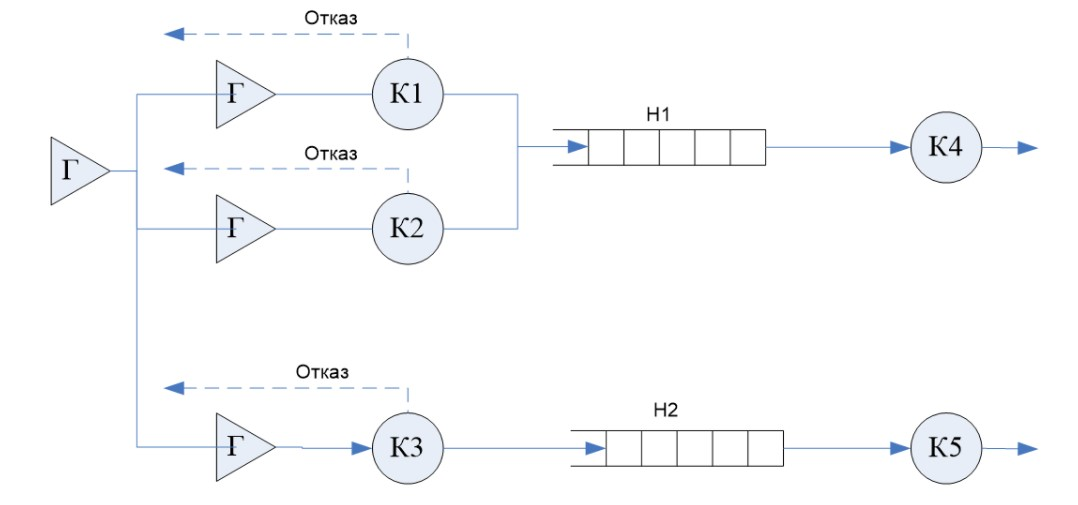
\includegraphics[scale=0.7]{task2.jpg}
				\caption{Структурная схема модели}
				\label{pic:scheme}}
		\end{center}
	\end{figure}
	
	Согласно условию время обработки заявки оператором подчиняется закону равномерного распределения, а время компьютер выполняет каждую обработку фиксированное время. Автоматы обслуживания в модели классифицируются следующим образом:
	\begin{itemize}
		\item K1, K2, K3 - АО, симулирующие работу операторов. Они является одноканальными системами с потерями и обозначаются как G/G/1/1.
		\item K4, K5 - АО, симулирующие работу компьютеров. Они является одноканальными системами с ожиданием и обозначаются как G/Д/1.
	\end{itemize}

	Эндогенными переменными системами являются время обработки заявки для операторов и компьютеров. Экзогенными являются число клиентов, которые были обслужены и число получивших отказ.

\section{Работа программы}	
	Результаты моделирования приведены на рисунке \ref{pic:res}.
	
	\begin{figure}[h]
		\begin{center}
			{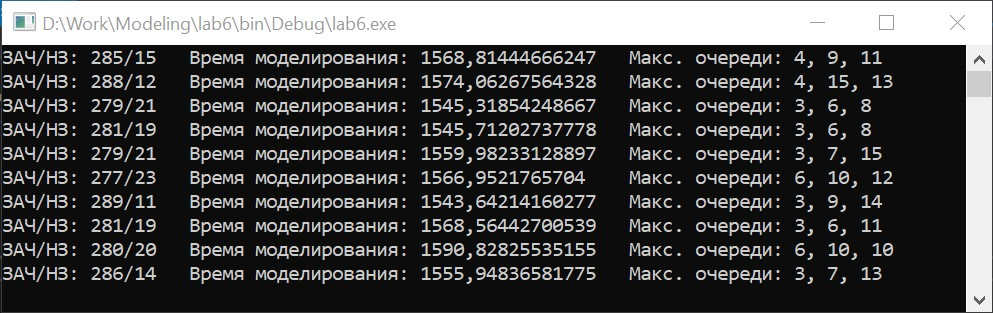
\includegraphics[scale=0.85]{result.jpg}
				\caption{Пример работы программы}
				\label{pic:res}}
		\end{center}
	\end{figure}
	